\documentclass[tikz]{standalone}

\usetikzlibrary{shapes.arrows}

\begin{document}
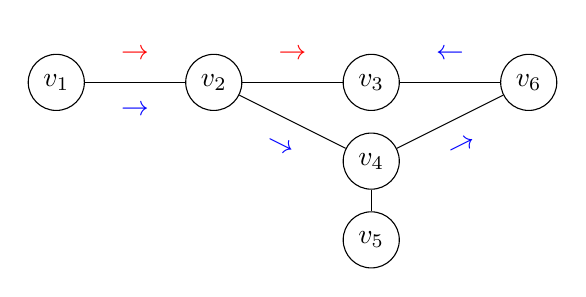
\begin{tikzpicture}[every node/.style={circle, draw}]
    \node (v1) at (0, 0) {$v_1$};
    \node (v2) at (2, 0) {$v_2$};
    \node (v3) at (4, 0) {$v_3$};
    \node (v4) at (4, -1) {$v_4$};
    \node (v5) at (4, -2) {$v_5$};
    \node (v6) at (6, 0) {$v_6$};

    \draw (v1) -- node[draw=none, above, red] {$\rightarrow$} (v2);
    \draw (v2) -- node[draw=none, above, red] {$\rightarrow$} (v3);
    \draw (v1) -- node[draw=none, below, blue] {$\rightarrow$} (v2);
    \draw (v2) -- node[draw=none, below, blue, sloped] {$\rightarrow$} (v4);
    \draw (v3) -- (v6);
    \draw (v4) -- (v5);
    \draw (v4) -- node[draw=none, below, blue, sloped] {$\rightarrow$} (v6);
    \draw (v6) -- node[draw=none, above, blue, sloped] {$\leftarrow$} (v3);
\end{tikzpicture}
\end{document}